\documentclass[10pt,conference]{IEEEtran}
%\documentclass[a4paper,12pt]{article}
%\usepackage{algpseudocode}
\usepackage{cite,latexsym,times,epsf,amsmath,amssymb,amsfonts,graphicx}
\usepackage{epstopdf}
\usepackage{graphicx}
\usepackage{subfigure}
\usepackage{multirow}
\usepackage{algorithmic}
\usepackage{algorithm}
\usepackage{amsmath}
\usepackage{verbatim}
\usepackage{booktabs}
\usepackage{authblk}
\usepackage{bm}
\renewcommand{\algorithmicrequire}{\textbf{Input:}}
\renewcommand{\algorithmicensure}{\textbf{Output:}}
\renewcommand{\baselinestretch}{0.915}
%\renewcommand{\algorithmicforall}{\textbf{Foreach}}
%\renewcommand{\algorithmicendfor}{\textbf{}}


\begin{document}
\title{WhiteCell: Energy-Efficient Use of Unlicensed Frequency Bands for Cellular Offloading}
\author{Pengfei Cui}
\author{Matthew Tonnemacher}
\author{Dinesh Rajan}
\author{Joseph Camp}
\affil{Department of Electrical Engineering, Southern Methodist University}
%\documentclass[10pt]{article}

%\usepackage{xkvltxp}


\maketitle


\begin{abstract}

%While many metropolitan areas sought to deploy city-wide WiFi networks, the densest urban areas were not
%able to broadly leverage the technology for large-scale Internet access.  Ultimately, the small 
%spatial separation required for effective 802.11 links in these areas resulted in prohibitively large up-front 
%costs.  

The FCC has reapportioned spectrum from TV white spaces for the purposes of large-scale Internet 
connectivity via wireless topologies of all kinds. 
The far greater range of these lower carrier frequencies are especially critical in dense areas, where 
high levels of aggregation could adapt the mobility of users.
However, the restriction of white space in dense area limits the available number of white space channels 
in dense areas. 
Thus, leveraging the range of spectrum across user mobility becoms a critical issue for the deployment of 
data networks with WiFi and white space bands. 
% Work
In this paper, we measure the spectrum utility in typical environment of the Dallas-Fort Worth metropolitan. 
We formulate the heterogeneous wireless network with both WiFi and white space bands as a queuing system. 
Further, we propose a measurement-driven resource allocation algorithm, Greedy Server-side Replace (GSR).
In particular, we study the white space and WiFi bands with in-field spectrum utility measurements, revealing 
the power consumption required for an area with channels in multiple bands. In doing so, we find that 
networks with white space bands in dense areas reduce the power consumption by up to FIXME 
% In sparse area, the power consumption is the most


\end{abstract}

\section{Introduction}
\label{sec:introduction}

%  Multiband background
The FCC has approved the use of broadband services in the white spaces of 
UHF TV bands, which were formerly exclusively licensed to television broadcasters.
These white space bands are now available for unlicensed public use, enabling the
deployment of wireless access networks. These white space bands operate in available 
channels from 54-806 MHz, having a far greater propagation range than WiFi bands for 
similar transmission power~\cite{balanis2012antenna}. 
% Improve existing cells
Thus, white space bands could greatly complement the existing WiFi wireless network with 
a large area. The users in the propagation range of the access point with white space radios 
has the options to associate with either the WiFi channel of its cell or the white space 
channel.



% Multi-user diersity
The users in multiple locations under the coverage of both the WiFi and white space have {\it user 
diversity}. The term user diversity represents the same frequency band at the same time can offer 
different transmission qualities to different users due to their difference in transceiver design, 
geographic location, etc.
% Explain the spectral diversity temporal diversity
The user diversity comes from two types of diversity gains. One is the temporal diversity which 
is caused by the environment variation. Another is the spectral diversity which represents the 
transmission conditions varies across channels. 
In some moderate number of users, the sum capacity of the fading channel is greater than 
the sum capacity of a nonfading channel. In the fading channels, the sum capacity of users 
increase with the number of users in the system~\cite{viswanath2002opportunistic,gan2014multiple}. 


% White space limited resource
%Moreover, the number of available white space channels are restricted by FCC. In sparse rural area,
%there are more free channels in white space. Inversely, few available channels are located in dense 
%populated area. The question {\it how limited white space resource befinet the access of the users 
%in these diversity scenarios?}

Previous work studied the multi user setting with a single channel~\cite{tan2010distributed}. Spectral diversity 
is isolated for a single user in~\cite{shu2009throughput}. In~\cite{liu2013stay}, multi-user dynamic channel access is 
proposed jointly consider the temporal and spectral diversity in a multichannel model. However, 
none of these works address the channel association problem in multiband scenario.

The larger propagation range of white space channels adapt channel association of users located 
in large area through time division. When the users distributed in a large area, the temporal 
diversity and spectral diversity become the key issues of white space applications.
Previous work~\cite{pcuiwinmee} studied the white space application in access network deployment 
with spectral diversity. However, these works fails to leverage the white space frequency in 
multi-user diversity in both spectral and temporal scenarios.

% Extreme cases and the middle
In sparse rural areas, plenty of white space channels are able to deploy new white space network. However, 
in dense area, few white space channels are available for new network deployment, such as none white 
space channel is available in New York downtown~\cite{googlespectrum}. The carrier have to use WiFi 
channels to deploy wireless networks in the dense area without any available white space channel. 
Other than these two extreme cases, most areas of major cities in the United States have one to eight 
white space channels~\cite{googlespectrum}. Exploiting these limited white space resource to improve 
the WiFi network in dense area is a perspective option for the dense areas.

% Power saving, extreme cases
The white space frequencies offer more wireless capacity and conienience of access across large 
area. When the traffic demands of the users are relatively low, a single white space channels satisfy 
all the user. Then, the WiFi radios could be turned off for saving power. On the other side, 
when the users have high traffic demand, all the radios, WiFi and white space, have to be operated to serve the users. 
However, traffic demands generally come across somewhere between these extremes.
Thus, the question comes out,a{\it in what degree the white space help to reduce the power consumptions of 
an existing WiFi mesh?} 

% Traffic Demand
In this work, we study channel schedule in a multi-user multiband setting, where users are not 
fully backlogged, traffic demand follow a certain arrival process. We focus on the effect of channel 
schedule of each user between the WiFi or white space band. 

% On demand consideration

% Paper contributions
In particular, the main contributions of our work are as follows:
%\begin{itemize}
%\item We perform the in-field measurements of user diversity in various representative scenarios 
%across the DFW metroplex.
%\item We formulate the channel association problem in multiband scenario.We develop a fixme
%algorithm to associate the users to the access points approaching the optimal effective rate.
%\item We design a payoff function to improve the fairness among the users and the quanlity of service.
%\item We analyze our algorithm with our in-field measurements to show that white space band 
%could improve 
%\end{itemize}
%
%The rest of the paper 

\section{System, Assumptions and Problem Formulation}
\label{sec:problemformulation}

% Background and problem model
\subsection{System and Assumptions}
\label{subsec:model}
% Background
% Multiband variation
Wireless propagation refers to the signal loss characteristics when wireless signals 
are transmitted through the wireless medium. The strength of the received signal depends on 
both the line-of-sight path (or lack thereof) and multiple other paths that result from reflection, 
diffraction, and scattering from obstacles~\cite{andersen1995propagation}. The widely-used Friis
equation characterizes the received signal power $P_r$ in terms of transmit power $P_t$, transmitter 
gain $G_t$, receiver gain $G_r$, wavelength $\lambda$ of the carrier frequency, distance $R$ from 
transmitter to receiver, and path loss exponent $n$ according to~\cite{friis}:
\begin{equation}
\label{eq:friis}
P_r=P_t+G_t+G_r+10n \log_{10}\left( \frac{\lambda}{4\pi R}\right)
\end{equation}
Here, $n$ varies according to the aforementioned environmental 
factors with a value ranging from two to five in typical outdoor 
settings~\cite{rappaport}.
% Tell the propagation of white space is much larger than wifi
Thus, the channels of low frequency white space bands propagates further than the high frequency WiFi 
bands with the same RSSI threshold, transceiver settings according to Eq.~\ref{eq:friis}. 
% White spcae is good out resource to improve the service of Wifi cell
The propagation range of low frequency white space channels is times of WiFi channels, for instance, 
450 MHz channels has more than 12 times propagation range as 5 GHz channels via Friis model. Thus a 
single white space access point is possible to serve an area up to hundreds times of a WiFi access point. 
The larger propagation of white space channels is potentially to be applied for reduction of network deployment 
cost~\cite{pcuiwinmee}, adaptation of vehicular dynamic access~\cite{chen2011feasibility}, and improvement 
of network capacity~\cite{bahl2009white}.
However, previous works focus on the application of plenty white space channels resource or point to point 
communication require small amount of white space resource. 


%FIMXE insert table tell the number of white space channels in US cities
\begin{table*}[hpt]
\centering % centering table 
\begin{tabular}{|l|c|c|c|c|c|c|c|} % 
\hline %\hline % inserting double-line 
City & New York & Log Angeles & San Francisco & Seattle & Houston & Austin & Dallas \\
\hline %\hline % inserting double-line 
White space channels & 0 & 0 & 2 & 7 & 3 & 1& 3 \\
\hline %\hline % inserting double-line 
\end{tabular}    
\caption{Number of White Space Channels in Major Cities} % title name of the table 
\label{tab:whitespacechannel}    
\vspace{-0.3in}
\end{table*}    

In wireless network design, as discuss in previous works, the more wireless channel resource means the better 
performance.
Unfortunately, FCC restricts the number of white space channels in most dense populated areas due to the existing 
TV broadcasting application. The minimum number of white space channels in major cities in the U.S is listed in 
Table~\ref{tab:whitespacechannel}.
There are areas has no white space channel available in New York and Los Angeles. 
Austin has only one white space channel available in downtown area.
The other cities in the table have 2 to 7 white space channels.
Thus, a heterogeneous network with WiFi channels and few white space channels 
becomes a practical option for these cities other than a white space wireless network.



% Power saving
\begin{figure}
\vspace{-0.0in}
\centering
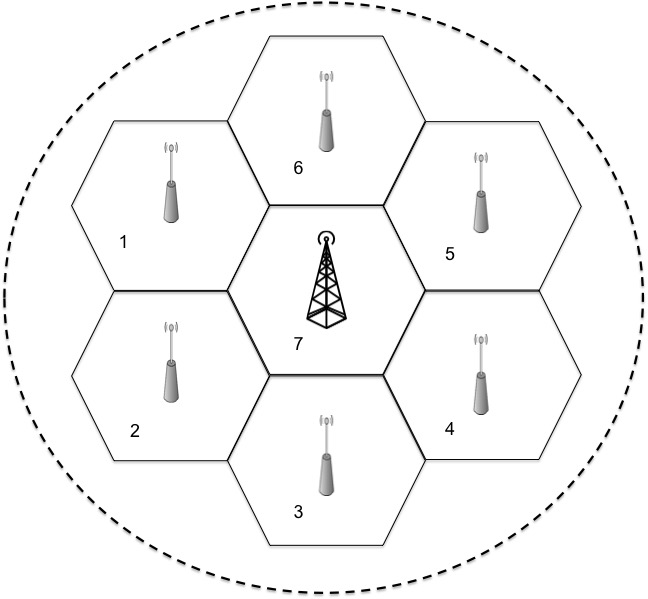
\includegraphics[width=84mm]{figures/whitecell}
\vspace{-0.1in}
\caption{Heterogeneous WhiteCell Structure}
\label{fig:systemmodel}
\vspace{-0.1in}
\end{figure}


% Give the model and assumption
% B channel; N user; M AP;
Here, we introduce a heterogeneous network named as WhiteCell with existing WiFi cells and an access point 
with few number of white space channels as shown in Fig.~\ref{fig:systemmodel}.
Given a WiFi mesh wireless system with $M$ access points and $N$ users.
The users in each WiFi cell of the network have access to the white space channels and the assigned WiFi channel of the cell. 
The reuse of WiFi channels has been discussed in plenty of previous works and it is out of our scope.
There are $F_w$ white space radios is installed on one of the access points to assistant the existing WiFi 
network. 
The capacity in clean environment of each radio $C$ is an equally restrict number for all the channels. 
There are enough buffer store the traffic demand from the users on each radio. 
The traffic is served in a first-in-first-out (FIFO) scheduling system. 
In such a network, each user has $1+F_w$ channels to be scheduled. One is the previous in-cell WiFi channel 
and the white space channels. 
We assume the users in the same mesh cell are in a single interference domain. 
Considering the limited number of white space channels in dense area and the fact spatial reuse 
of white space will make the problem considerably more challenging, we will remains an interesting 
direction of future research. 


Instead of assuming the wireless channels are on-off~\cite{bodas2012low} or equally clean, we apply a  
measurement method to get the achieved channel capacity. The capacity of the channel between the access 
points and users is noted as a matrix in Eq.~\ref{eq:usercapacity}
\begin{equation}
\label{eq:usercapacity}
H_{i,j}^f(t)= G(\zeta,t),i \in M, j\in N, f \in (F_M+F_w) 
\end{equation} 
$\zeta$ represents the in-field measured historical data and dynamic sensing information.
We use a context-aware method to estimate the $j$ user capacity $H_{i,j}^f(t)$ to an access point 
$i$ on channel $f$. The users in a single cell has the same channel status. We assume the channel 
capacity is flat during a time slot. The switching time is negligible in the system.
The calculation of achieved channel capacity is introduced in~\ref{subsec:experimentsetup}. 
The traffic demand arrive at a user as a Poisson process, with the vector noted as 
$\bm{D(t)} = [D_1(t),D_2(t),...D_N(t)]$ and the sum rate $D(t) = \sum\limits_{i=1}^N D_i(t)$. 
The rate $D(t)$ is the aggregate rate of data generated from all users. 

% Buffer and tolerance time
During a time slot, the unscheduled radios remain in sleep mode to save energy. Also we ignore 
the sleeping energy as well as the amount of energy spent on channel/radio switching. An operating 
radio will cost equal power in a time unit. Previous work~\cite{niida2010user} shows a user has a 
certain patience for waiting. The tolerance time varies across the traffic type, such as text information, 
voice information. To simply the problem, we assume an average value for $W$ of all the users in the system. 
The smaller tolerance time of the users, the more channel capacity resource is required.
The system applies a first-come-first-serve schedule. The white space channels are able to split for multiple 
cells.

\subsection{Problem Formulation}
\label{subsec:problem}

We formulate the system introduced in~\ref{subsec:model} as a discrete-time queuing system as shown in 
Fig.~\ref{fig:flowconfig}. 
The channels are represented as servers in the queuing system. 
% Do we need it?
Table.~\ref{tab:notation} summarizes the notation used in this work. 
The system has $F_w$ white space channels, $F_M$ WiFi channels in total and $N$ users.
Thus, the queuing system has $N$ queues and $F_M+F_w$ servers connecting by time-varying 
channels $H^*(N,F_M+F_w)$.

\begin{table}[htbp]
\begin{center}% used the environment to augment the vertical space
% between the caption and the table
\begin{tabular}{l l p{10cm} }
\toprule
$t$ & Time slot\\
$N$ & Set of users\\
$M$ & Set of Access points\\
$H_{ij}^f$ & Measurement based Capacity between AP i and user j on channel f\\
$F_{m}$ & WiFi Channels with Access Points\\
$F_{w}$ & Set of White Space Channels\\
$A(t)$ & User access channel schedule\\
$B$ & User Buffer\\
$C$ & Radio Capacity\\
$R$ & Operating Radio\\
$\zeta$ & In-Field Measurements\\
$W$ & Tolerance time window \\
%$R_{i}$ & $\triangleq$ & Revenue at store $i$\\
%$i$ & $\triangleq$ & index value for store locations\\
%${T}_{c}$ & $\triangleq$ & A very long description of this specific variable and is needed in the research and looks good when wrapped and aligned to the left.\\
%$TC$ & $\triangleq$ & Total overall cost(\$)\\  
%\multicolumn{3}{c}{}\\
%\multicolumn{3}{c}{\underline{Decision Variables}}\\
%\multicolumn{3}{c}{}\\
%$y_f$ & $=$ & \(\left\{\begin{array}{rl}
%1,  & \text{if Supplier located at site $f$ is open} \\
%0,  & \text{otherwise} \end{array} \right.\)\\
\bottomrule
\end{tabular}
\end{center}
\caption{Table of Notations}
\label{tab:notation}
\end{table}



\begin{figure}
\vspace{-0.0in}
\centering
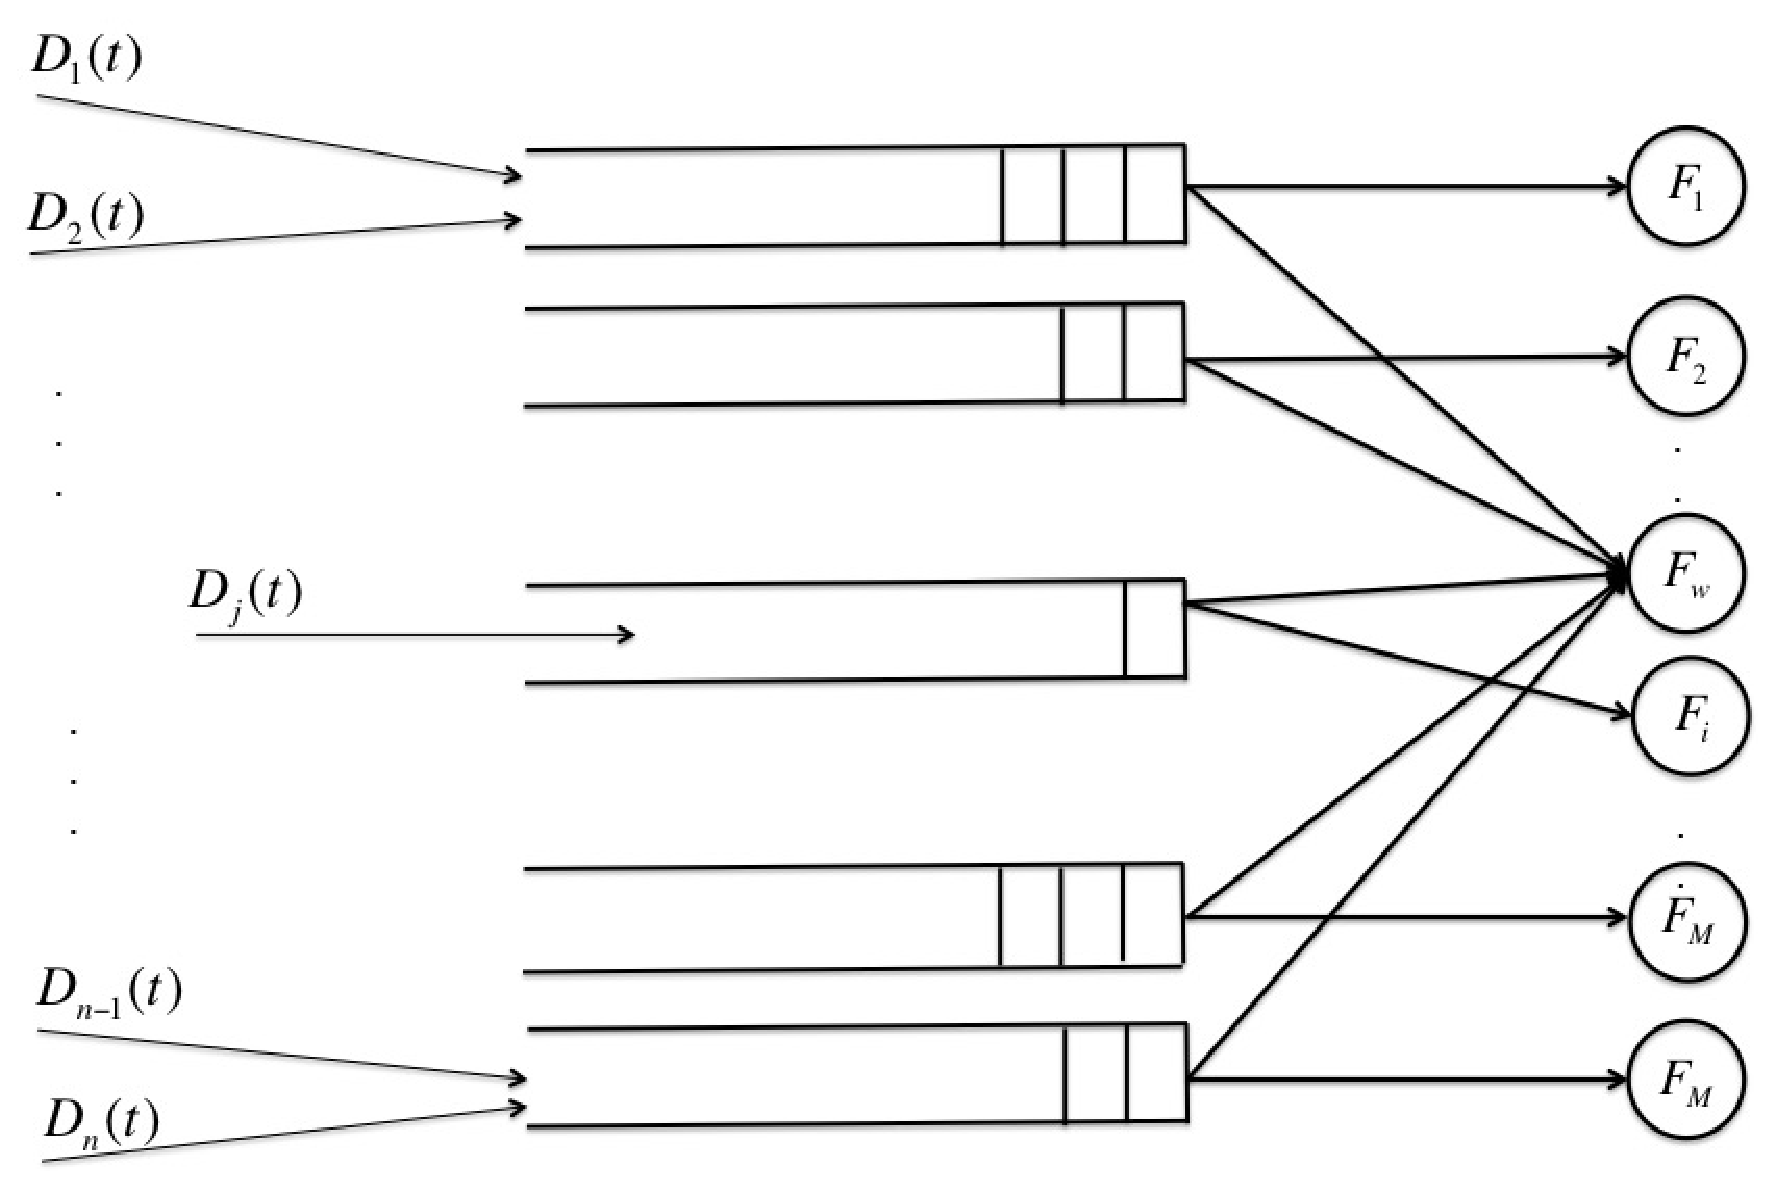
\includegraphics[width=84mm]{figures/flowconfig}
\vspace{-0.1in}
\caption{System Model}
\label{fig:flowconfig}
\vspace{-0.1in}
\end{figure}

Let matrix \{$A_{i,j}(t),i\in (F_M+F_w), j\in N$\} denote the associate meets the 
tolerance constraint as shown in Eq.~\ref{eq:associate_def}.
%where $A_{i,j}^b = 1$ denotes user $j$ is scheduled with access point $i$ on channel $b$.
\begin{equation}
\label{eq:associate_def}
 A_{i,j}(t) = \left\{ 
	  \begin{array}{l l}
	    1   &  if\ D_{j\in N},\ is\ associated\ with\ \\
		& channel\ i \in (F_M+F_w) \\
		0 &  Otherwise
			    \end{array} \right.
\end{equation}

The queuing system keeps the expected waiting time of the system $w$ less than the tolerance threshold $W$ 
as shown in Eq.~\ref{eq:timeconstraint}
\begin{equation}
\label{eq:timeconstraint}
E[w]\le W
\end{equation}

With the intuition, when the total traffic demand of the users in the system are relatively small, a single 
white space channel could achieve the quality of service for the users. Thus all the WiFi radios could be turned 
into sleep mode for power saving. 
On the other side, as the traffic demand increase with the number of users or the demand per user, we need 
to increase the channel resource as servers in the system to qualify the user waiting time tolerance requirements. 
Moreover, when the users are distributed non-uniformly, the white space channels are able to deliver more capacity for 
the cells with more users to balance the system load without new infrastructure. 
The flexibility of white space channels offers new opportunity for network design.
To apply these white space advantages, the question {\it how much power we could save via dividing the white space 
capacity into the WiFi cells?} has to be addressed in this system.

In this work, we focus on the analysis on the power consumption saving of the heterogeneous wireless system. 
To model the power consumption of the system, we count the power consumption of each operating radio via 
standby and transmitting power consumption.
We assume the sleeping standby power consumption is negligible. 
We define $R_i$ represents the radios status in the system, $i\in {F_w,F_M}$. 
When $R_i$ is working in WiFi channels $F_M$ or white space channels $F_w$, $R_i$ denotes the power consumption 
with the standby and transmitting cost. 
Otherwise, $R_i = 0$. The definition is as shown in Eq.~\ref{eq:radio}

\begin{equation}
\label{eq:radio}
 R_i(t) = \left\{ 
	  \begin{array}{l l}
	    P_s+P_t\cdot\mu   &  \sum\limits_{j=1}^N A_{i,j}(t) \ge 1\\
		0 &  Otherwise
			    \end{array} \right.
\end{equation}

% Explain the equation
$P_s$ is the constant standby power consumption of a radio, $P_t$ is the transmit power for the channel capacity 
assigned of the radio. $\mu$ is the total assigned channel capacity of the radio.
$R_i(t)$ is the power consumption of the radio in the time slot.

Thus, to reduce the power consumption, we need to minimize $R_i$ for all the radios under the quality of service 
constraints. 
Our goal, to minimize the power consumption is represented in Eq.~\ref{eq:objective}:
\begin{equation}
\label{eq:objective}
R^*(t) = \min{\{\sum\limits_{i=1}^{(F_M+F_w)} R_{i}}(t)\}
%\xi = \min{\{\sum\limits_{t}^{t+T}\sum\limits_{i}^{(F_M+F_w)} R_{i}}(t)\}
\end{equation}
$R^*$ represent the minimum operating radios power consumption required for the system. 


% Background and problem model
\subsection{Challenges And Analysis}
\label{subsec:challenge}
% Challenges sum
Prior works model similar multi-channel system as $M/M/m$ queuing system for analyzing~\cite{bodas2012low}.
However, this system is not able to be formulated as a $M/M/m$ queuing system due to the 
non-equal capacity of the assigned channel capacity across white space and WiFi channels.
Thus we first analyze the queuing system and apply previous work in $M/M/m$ queuing theory to 
generate the solution for such system.

% introduce the queue system
Without the white space channels, the users in a cell can only access to the WiFi channel assigned for the 
cell to get service. The large propagation of white space channels offers more options for all the users. 
The user could either associate with the white space channels or the WiFi channels. 
Thus, the white space channels could be splited into several cells. 
The spliting of the white space channels brings more capacity variation of the servers. 
The white space channel spliting capacity variation and the spectrum capacity variation of cells might remove the 
equal service capacity assumption of the system in most scenarios.
However, the equal server capacity is the pre-request for a general $M/M/m$ queuing system analysis.
Thus, the $M/M/m$ queuing system of a multi-channel version is not directly applicable for this system model.



% User constraints
In the design of the wireless system, the response time $W$ constraints have to be satisfied to keep the 
quality of service. 
The users in this system can only be served by the large propagate white space channels or the WiFi 
channels assigned in the cell. 
% User diversity
The users located in multiple cells have different channel status in the same white space channels, 
which is mentioned as part of the multi-user diversity in previous works. Multi-user diversity is a 
form of diversity inherent in a wireless network, provided by independent time-varying channels across 
the different users~\cite{viswanath2002opportunistic}. 
The diversity could be generated by the interference from device inside the network or out of the network, 
the environmental variations.  
% Channel capacity diversity
The variation among users make the channel capacity among all the cells for white space channels. 
Thus, some cells may have clean white space channels in the air while the other cells may suffer 
worse white space channel performance. 
To address the variation, instead of holding the on-off channel assumption, we implement an in-field 
measurements based channel capacity estimation approach in this work.

% Activity level instruction
We define an activity level to estimate the achieved channel capacity. 
We perform measurements to sense the activities in the air through our portable spectrum analyzer.
The percentage of sensing samples ($S_\theta$) above an interference threshold ($\theta$) over the 
total samples ($S$) in a time unit is the activity level ($A$):
\begin{equation}
\label{eq:actdef}
A=\frac{S_\theta}{S_a}
\end{equation}
The capacity of a clean channel is denoted by $C$. With the protocol model, the achieved capacity 
of a channel $C_r$ could be represented as the remaining free time of the channel capacity 
according to Eq.~\ref{eq:intercap}: 
\begin{equation}
\label{eq:intercap}
C_r=C*(1-\bar{A})
\end{equation}

% User distribution measurements
Other than the achieved channel capacity, we also perform in-field measurements of the user mobility footprint. 
When the total number of the users is a certain value, the user distribution becomes important for wireless network 
operating. We analyze the dataset from WiEye, an Android application reports the location, velocity and signal 
information to leverage the mobility pattern of users during week days. The setup and results are shown in 
Section~\ref{sec:experiment}.

% analysis
With thses measurements information, we further analyze the channle capacity allocation for such a system. 
We first investigate the channel capacity allocation in a single cell.
The users of the the same WiFi cell are in a heterogeneous queuing system with server of 
WiFi channels and white space channels with service rate $\mu_1,\mu_2,...\mu_{(F_w+1)}$.
$\mu$ denote the capacity allocated for this cell.
The white space channel capacity is splited into multiple WiFi cells, thus, the 
capacity of the white space is usually the minimum channel capacity in a cell.
Thus, there are three cases of the channel capacity in a single cell. 
The first scenario is several channels of both WiFi and white space works for the cell and the capacity of some 
white space channel is several time less than other channel capacity since white space channels are splited 
for many cells. 
An example here is in a single cell, the white space channel assigned is equally distributed to two cells, while 
the WiFi channel works in this cell, thus, the capacity of the WiFi channel is about twice of the white space 
channel capacity in this cell.
The second scenario is only the WiFi channel or only part of a single white space channel works 
for the cell. 
The third scenario is several channels work for this cell with around equal capacity.
The fist case is a heterogeneous server queuing system with inequal capacity servers.
The second case is simplified as a $M/M/1$ queuing system. 
The third case is converted into a $M/M/m$ queuing system.

For the first case heterogeneous server queuing system, we apply the transformation model 
in~\cite{yu2008transformation} to estimate the response time $\bar{w}$. 
In the transformation model, the actual arrival rate for one specific server $\lambda_s$ is 
defined as in Eq.~\ref{eq:actarrivalrate}
\begin{equation}
\label{eq:actarrivalrate}
\lambda_s=D_{cell}/(F_w+1)
\end{equation}
$D_{cell}$ is the traffic aggreated from the users in the cell.

The other parameters are noted from Eq.~\ref{eq:transformation} to~\ref{eq:kvalue}.
\begin{equation}
\label{eq:transformation}
\mu_{min}=\min{(\mu_1,\mu_2,...\mu_{(F_w+1)})} = \bar{\mu}
\end{equation}

\begin{equation}
\mu_{max}=\max{(\mu_1,\mu_2,...\mu_{(F_w+1)})} 
\end{equation}

\begin{equation}
\label{eq:kvalue}
k= \lfloor\frac{\mu_{max}}{\mu_{min}} \rfloor
\end{equation}

When $k=1$, the system becomes a homogeneous queuing system as in case three. Otherwise,   
$k\ge2$ the average response time of such heterogeneous system could be represented as in 
Eq.~\ref{eq:heterresponse}\cite{yu2008transformation}:

\begin{equation}
\label{eq:heterresponse}
\bar{w}=\frac{1}{\frac{1}{3}\bar{\mu}(2k+1)-\lambda_s}
\end{equation}

Through the transformation model, we could further calculate the channel capacity required for 
response time constraints. Further, the power consumption could be calculated for the system.
When the traffic could be served by part of a single white space channel or the WiFi channel, as 
the second scenario, the system converge into a $M/M/1$ queue. The response time $\bar{w}$ 
could be estimated from Eq.~\ref{eq:mm1w}~\cite{gelenbe1998introduction}.

\begin{equation}
\label{eq:mm1w}
\bar{w}=\frac{1}{\mu^+-D}
\end{equation}
$\mu^+$ is the channel capacity of the single channel capacity in queuing system.

% Here
In the third scenario, the system could be treated as a $M/M/m$ queuing system. 
The average reponse time is calculated as in Eq.~\ref{eq:mmmw}~\cite{gelenbe1998introduction}.
\begin{equation}
\label{eq:mmmw}
\bar{w} = \frac{1}{\mu^*}(1+\frac{c(m,\rho)}{m(1-\rho)})\approx \frac{1}{\mu^*}\frac{1}{1-\rho^m}
\end{equation}
$\mu^*$ is the average capacity of channels in the $M/M/m$ queuing system.
$\rho=\frac{\lambda}{m\mu^*}$ is the traffic density, and $c(m,\rho)$ is the Erlang-C 
formula~\cite{gelenbe1998introduction}.



In this model, the less radio in operation and the less power consumption will be cost in the system according to 
Eq.~\ref{eq:radio}. 
The basic idea of power reduction for this heterogeneous system is to replace the WiFi radios via white space channel 
capacity. To implement the division of the white space capacity we propose a Greedy Server-side Replace(GSR) algorithm 
to approach the minimize power consumption in the system as shown in Algorithm~\ref{algorithm:gsr}. 

\begin{algorithm}[t]
\small
\caption{Greedy Server-side Replace}
\label{algorithm:gsr}
\begin{algorithmic}[1]
\REQUIRE  ~~\\
$N$: Users\\
$H_{i,j}^f$: Vector of channel capacity\\
$D$: Traffic Rate\\
$n$: Path Loss Exponent \\
$M$: WiFi Cells
\STATE {Find the WiFi cell with the lowest traffic rate $D$,break the tie with index}
\STATE {Calculate the power consumption according to Eq.~\ref{eq:heterresponse}~\ref{eq:mm1w}~\ref{eq:mmmw}}
\IF {If channel resource feasible}
\STATE {List available options}
\IF {Single channel is the best}
\STATE Apply half-interval search to find the minimum capacity for the users
\ELSIF {Homogeneous is the best}
\STATE Allocate the resource for the cell
\STATE Keep the WiFi channel and find the minimum capacity for the users
\ELSIF {Heterogeneous is best}
\STATE Adding white space resource to the cell
\ENDIF
\ELSE 
\STATE Get the waiting time of the cell with all available resource
\ENDIF
\STATE Update the system information
\STATE Repeat the process for all the cells
\STATE Calculate the power consumption
\ENSURE ~~\\
The power consumption and the maximum waiting time\\
\end{algorithmic}
\end{algorithm}


% Here, introduce the algorithm
%Fixme
We integrate the in-field measured data To answer the design question, we first get the channel capacity from the in-field measurement, then we 
propose a Greedy Server-side Replace (GSR) algorithm to minimize the power consumption and achieve the 
performance constraints.




% Fixme the capacity from activity level
The calculation of channel capacity $H$ will be discussed in Section~\ref{sec:experiment}.
The algorithm starts to reduce the standby power then the transmitting power for each server.





The algorithm output the channel resource allocation to satisfy the waiting 
time constraint of the system.




\section{Experiment and Analysis}
\label{sec:experiment}

In this section, we introduce the measurements experiments setup and 
evaluate the process of probabilistic forecasting of channel state.

% Subsec Experiment design
\subsection{Measurements}
\label{subsec:measurements}

% 24 hours measurement introduction
We perform measurements in neighborhoods, campus, downtown bussiness office and 
urban bussiness office for 24 hours on weekdays. 
The locations we chosen for measurements are shown in Fig.~\ref{fig:measurements}.

% Experiment equipment
We employ a Rohde \& Schwarz FSH8 portable spectrum works from 100 KHz to 8 GHz. 
The portable spectrum analyzer is controlled by a Python script on a laptop to measure 
the received signal strength.
% Data normalize 
To the best of our knowledge, there is no readily available mobile, multiband antenna from
450 MHz to 5.2 GHz on the market. Thus, we use a 700-MHz mobile antenna to perform in-field
measurements. We then normalize the mobile antenna performance across bands with indoor 
experimentation. To do so, we use a Universal Software Radio Peripheral (USRP) N210 to 
generate signals at 450 MHz, 800 MHz, and 2.4 GHz. We feed the USRP signals directly
to a spectrum analyzer and adjust the configuration of USRP to make the received signal 
strength the same as the 5.2 GHz signal from Gateworks 2358 with a XR5 radio. Then, we connect 
the signal source to a fixed multiband antenna (QT 400 Quad Ridge Horn Antenna) and measure the
received signal at a fixed distance with the 700 MHz antenna and antennas for different bands
to obtain the antenna loss for each band. We adjust the received signal strength
collected via the 700-MHz mobile antenna according to the normalization.

% Introduce how to calculate the capacity
% Explain multiband and activity level
When wireless devices operate in WiFi bands, the channel separation is relatively 
small (e.g., 5 MHz for the 2.4 GHz band). As a result, many works assume that
the propagation characteristics across channels are similar. However, with the
large frequency differences between WiFi and white space bands (e.g., multiple GHz),
propagation becomes a key factor in the deployment of wireless networks with both bands.
Here, a frequency band is defined as a group of channels which have
little frequency separation, meaning they have similar propagation characteristics.
In this work, we consider the diverse propagation and activity characteristics
for four total frequency bands: 450 MHz, 800 MHz, 2.4 GHz, and 5.2 GHz.
We refer to the two former frequency bands as white space bands and
the two latter frequency bands as WiFi bands.
The differences in propagation and spectrum utilization create opportunities
for the joint use of white space and WiFi bands in wireless access networks according
to the environmental characteristics (e.g., urban or rural and downtown or residential)
of the deployment location.


For spectrum utility and resulting channel availability, 
we split the measurements every 30 minutes of each band.  We define the percentage of sensing 
samples ($S_\theta$) above an interference threshold ($\theta$) over the total samples ($S$) in 
a time unit as the activity level ($A$) of inter-network interference:
\begin{equation}
\label{eq:actdef}
A=\frac{S_\theta}{S_a}
\end{equation}
The capacity of a clean channel is denoted by $C$. With the protocol model, the capacity 
of a channel with inter-network interference $C_r$ could be represented as 
the remaining free time of the channel capacity according to: 
\begin{equation}
\label{eq:intercap}
C_r=C*(1-\bar{A})
\end{equation}


% Need to discuss the \mu mapping with these measurements stuff



\subsection{Experiment Setup}
\label{subsec:experimentsetup}
















\subsection{Results and Analysis}
\label{subsec:results}



\section{Related Work}
\label{sec:related}


% White Space
Since white space bands were free for wireless communication, many efforts have been 
put in the area for the application of white space bands.~\cite{fccwhitespace} 
In~\cite{bahl2009white}. the author considered a cognitive method to avoid collision 
between white space communication and TV broadcasting. 
Many works increasing the convenience of using white space databases have been published 
(e.g., Microsoft's White Space Database~\cite{msdatabase}).
Google has even visualized the licensed white space channels 
in US cities with an API for research and commercial use~\cite{googledatabase}.
Previous work discussed the point to point communication with white space bands~\cite{cui2013leveraging}, 
and the wireless network deployment with plenty white space channels~\cite{pcuiwinmee}.
However, many of the major cities in the US do not have plenty white space channels, such as 
most area of Austin, TX has only one white space channel. As far as we know, there is no work 
discuss these scenarios.


%  Multi-channel
Applying white space in wireless network is similar to the previous multi-channel works other the 
propagation variation. In~\cite{bodas2012low} a multi-channel system is formulated as a queuing 
system and Server Side Greedy algorithm is proposed to optimize the throughput with low complexity. 
In~\cite{ji2013performance}, Delay-based Queue-Side-Greedy algorithm is proposed with low complexity 
for optimal throughput and near-optimal delay.~\cite{liu2014energy} develop a multi-objective optimization 
framework to minimal energy consumption in a multi-channel multi-radio system. 
However, these works do not address minimizing the resource for certain quality of service and assume an 
on-off channel model.

%% Multithread
% On-off channel
Previous works in real time systems put many efforts to minimize the resources, such as processors~\cite{nelissen2012techniques}.
In~\cite{li2014analysis}, the author proves the capacity augmentation bounds for schedulers of parallel tasks. 
However, these works assume the parallel tasks have uniform servers. 
Previous work~\cite{chen2011feasibility} investivate the white space in a queuing system without considering the 
hetergeneous topology.
In contrast, we study the performance of a hetergeneous network with both white space channels 
and WiFi channels in channel utilization. 

% gan2014multiple

% weighted sum/less info





\section{Conclusion}
\label{sec:conclusion}
In this paper, we considered the use of a small number of white space channel resources for reducing power consumption across a broad range of user mobility patterns and population densities. 
Towards this goal, we propose a heterogeneous wireless network and model it as a queuing system for additional analysis based on previous queuing theory work. 
To efficiently utilize the white space channels, we proposed a Greedy Server-side Replacement algorithm to allocate resources such that the power consumption in the network is minimized. 
We then performed spectrum utilization measurements in the several distinct locations including a downtown area, urban neighborhood, campus, and suburban neighborhoods to evaluate our algorithm. 
% Fixme
We leverage the impacts of channel quality, user mobility, quality of service, and population density on the network offloading structure. 
Further we investigate the performance in a virtual city to simulate the expected in-field performance. 
Through this simulation, we show that using white space channels can greatly reduce the power consumption of such offloading systems in most scenarios. 
From our results, we also see the advantage of using white space channels in adapting user mobility to reduce power consumption. 
% end
Through extensive analysis of spectrum utilization and user mobility, we showed that white space bands can reduce the average power consumption in white space heterogeneous networks by 64.70\% on average over 24 hours. 
Finally, we integrated previous measurements work in north Texas and find the power consumption is reduced by white space bands by 512.55\% in sparse area.
In the future, we will extend our work to include large scale user mobility patterns in addition to spectral activity levels for heterogeneous wireless network deployment optimization.
% Future work



\bibliographystyle{IEEEtran}

\bibliography{whitecell}

\end{document}
